%/*****************************************************************************
% * Download Elevation File
%/*****************************************************************************

\documentclass[12pt]{article}
\usepackage{float}
\usepackage{graphicx}
\usepackage[margin=1in]{geometry}

\graphicspath{{images/}}

\usepackage[utf8]{inputenc}
\usepackage[english]{babel}
\usepackage[parfill]{parskip}
\usepackage{datetime}
\usepackage{hyperref}
\hypersetup{
	colorlinks=true,
	urlcolor=blue,
  }
\urlstyle{same}
\usepackage{subcaption} 
\usepackage{dirtytalk}
\usepackage{multirow}
\usepackage{booktabs}


\usepackage{fancyhdr}
\pagestyle{fancy}
\fancyhf{}
\rhead{How to download an elevation file using WindNinja}
\cfoot{\thepage}

\newcommand\vn{3.4.0}

\begin{document}
\begin{titlepage}
    \centering
    {\Huge
       How to download an elevation file using WindNinja
    }    
    \vfill
    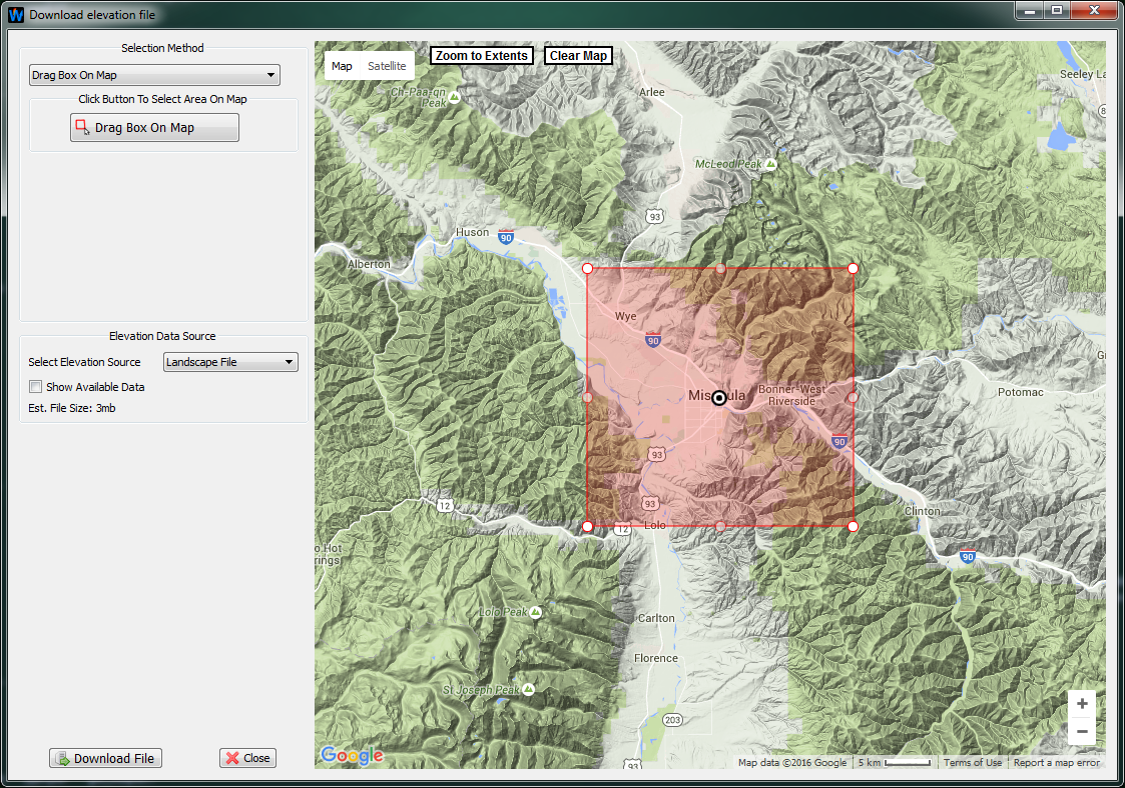
\includegraphics[scale=0.75]{dem_download_0}
    \vfill
  	{\Huge
	  7/02/2018 %Date Last Edited
  	}
    \vfill
\end{titlepage}


\section*{Introduction}
This document describes the functionality built into WindNinja to download
elevation files for wind modeling.  We call this utility the “elevation file
grabber”.  It allows you to use a custom Google Maps\texttrademark interface to zoom into
and select a desired area for wind modeling. The elevation data for this area
is downloaded by WindNinja from a USGS server and saved to a file on your
computer.  There is also a command line version of the elevation file grabber
that is described \href{http://firelab.github.io/windninja/pdf/fetch_dem_instructions.pdf}{here}.  The specific
options available and work flow are described below.

To open the elevation file grabber window, start WindNinja and click \textit{Surface Input} in the navigation tree at the top of WindNinja, then click the \textit{Download File} button as shown below.

\begin{figure}[H]
	\centering
	\label{}
	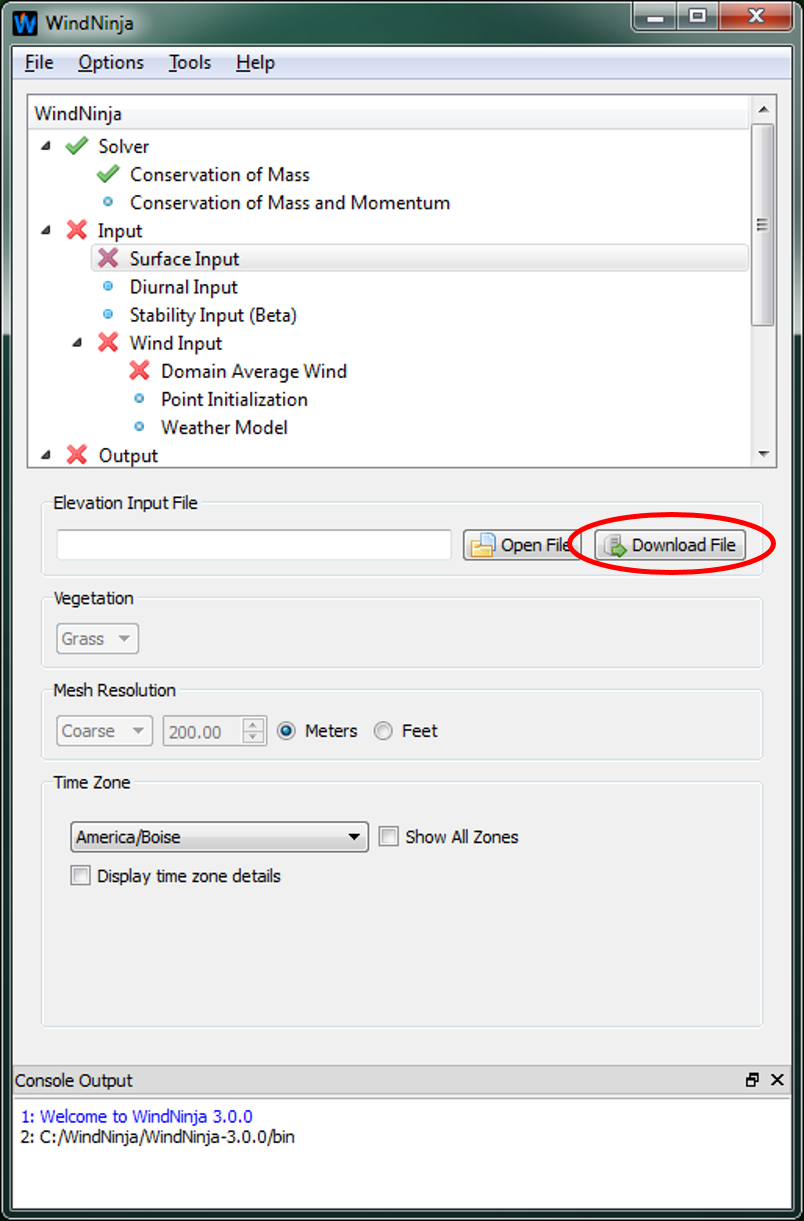
\includegraphics[scale=0.75]{main_window_0}
\end{figure}
\newpage

The \textit{Download Elevation File} window will open.  This window is divided into two areas as highlighted in red in the image below.  These areas are discussed in the next two sections.

\begin{figure}[H]
	\centering
	\label{}
	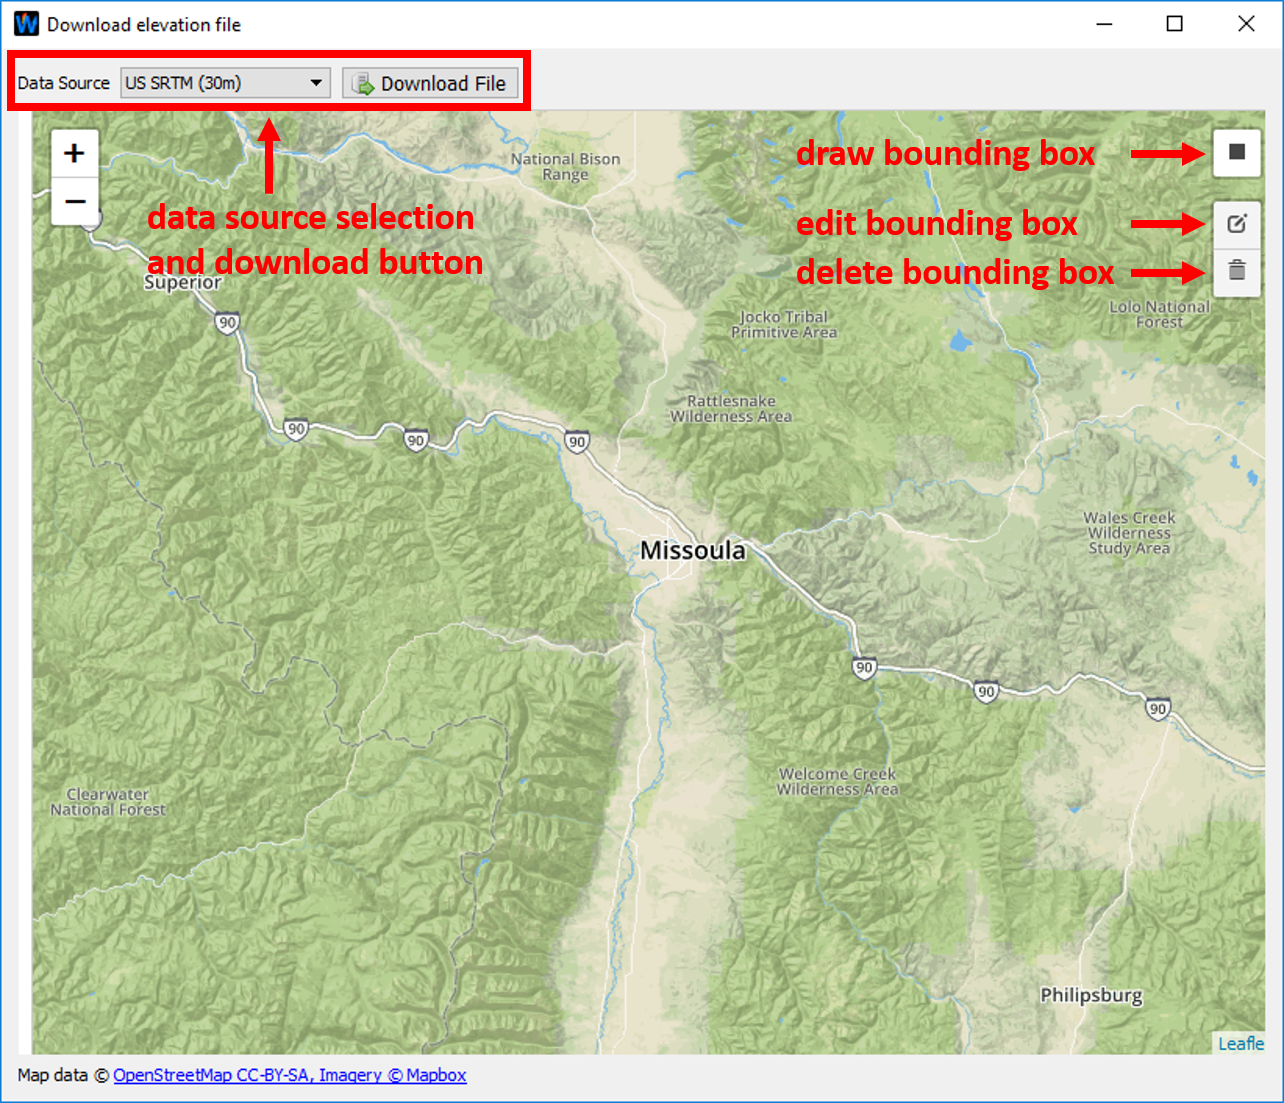
\includegraphics[scale=0.75]{dem_download_1}
\end{figure}

\section*{Graphics Window}
The graphics window is an interactive mapping display used to navigate into the desired wind simulation area.  This window uses a customized version of the popular Google Maps\texttrademark  software.  Various different base maps are available using the \textit{Map} and \textit{Satellite} buttons in the upper right corner.  There are a couple of ways to pan and zoom the map.  Using a mouse, you can pan with the left button and zoom using a mouse scroll wheel.  The keyboard can also be used to pan (arrow keys) and zoom (plus and minus keys).


\section*{Input Panel}
\subsection*{Selection Method}
%Below the 'Go To:' text box is the Selection Method group of buttons and text boxes that allow you to define the area you want to download.  This download area is a rectangular box that will be drawn over the map in the graphics window.  There are four different ways to define this rectangular box that can be chosen from the drop-down box.  They are:

The \textit{Selection Method} section of the input panel allows you to define the area that you want to download. This download area is a rectangular box that will be drawn over the map in the graphics window.  There are four different ways to define this rectangular box that can be chosen from the drop-down box.  They are:

\begin{enumerate}

\item \textbf{Drag Box On Map} \newline
	By clicking the \textit{Drag Box On Map} button, you can then left-click and drag on 		the graphics window to define a box of the desired size.

\item \textbf{Enter Bounding Box}\newline
	This option allows you to enter the latitude and longitude bounds for the box.
 
\item \textbf{Click Center Point} \newline
	This option allows you to click a center point on the map to define the center of the 		box and then enter the size of the box.
	
\item \textbf{Enter Center Point} \newline
	With this method, you enter the center point coordinates of the box and the box size.
\end{enumerate}

After using any of the methods above, a transparent red box will be drawn in the graphics window showing the area you've defined.  If you want, you can enlarge or shrink this box in the graphics window by dragging the sides or corners.  You can also move the box by dragging the center icon.  The \textit{Zoom To Extents} button in the graphics window will zoom the view to fit the box. The \textit{Clear Map} button will clear the box.

\subsection*{Elevation Data Source}

There are 4 possible on-line data sets to download elevation data from.  These are listed in the \textit{Select Elevation Source} drop-down box.  The main difference between these data sets is the spatial resolution and extent.  The table below briefly describes these differences.  You should be sure to choose a data set that covers your simulation area.

\begin{center}
    \begin{tabular}{| l | l | p{1.75in} | p{1.8in} |}
    \hline
    Data set name & Resolution & Spatial Extent & Description \\ \hline

    US SRTM & 30 meters  & Contiguous US, Hawaii, PR, Southern Alaska &
    Data from the Shuttle Radar Tomography Mission (SRTM) \\ \hline

    WORLD SRTM & 90 meters & Between approximately -60 and +60 latitude &
    Data from the Shuttle Radar Tomography Mission (SRTM) \\ \hline

    WORLD GMTED & 250 meters & Between approximately -60 and +85 latitude &
    Global Multi-resolution Terrain Elevation Data 2010 (GMTED 2010) \\ \hline

    Landscape (LCP) & 30 meters & Contiguous US, Hawaii, PR, Southern Alaska &
    FARSITE Landscape files including vegetation information \\ \hline
\end{tabular}
\end{center}
You can check the \textit{Show Available Data} check-box to display a blue polygon on the map outlining the chosen data set's extents.

\section*{Download The File}
Once you have defined your download area and selected the elevation data source, click the Download File button at the bottom to download the elevation file.  A window will open to allow you to specify a file name and location.  %The downloaded file is a geotiff file (*.tif) in best fit UTM projection using WGS84.
If you chose the option \textbf{US SRTM}, \textbf{WORLD SRTM}, or \textbf{WORLD GMTED}, the downloaded file will be a GeoTIFF (*.tif). \textbf{Landscape} files are downloaded as a .lcp file.
After the file is successfully downloaded, you can close the Download elevation file window and the downloaded file will be automatically loaded into the main WindNinja window.


\end{document}